
\chapter{Marco Teórico}

\label{chap2:marco-teorico}

\section{Introducción}

\label{sec21:introduccion}En este capitulo, se resumen las cuatro
áreas principales de estudio relacionados a los sistemas \abbr{HAR}
con miras a definir el problema del reconocimiento de actividades
humanas desde un punto de vista teórico. La descripción de estas áreas
detallan las aplicaciones que motivan los sistemas \abbr{HAR} y también
los mecanismos que llevan a una implementación factible. 

La primera sección, se introducen las aplicaciones de contexto que
son el principal marco de trabajo del estudio de sistemas \abbr{HAR}.
En síntesis, nuestro enfoque es detectar las actividades físicas para
dar información de contexto en las actividades diarias de un individuo
durante su locomoción. Las siguientes secciones dan todos los elementos
requeridos para implementar los sistemas \abbr{HAR}. Desde el punto
de vista de implementación se discuten los sensores y los teléfonos
móviles inteligentes. La última sección define el marco teórico del
reconocimiento de actividades humanas en base al estado de arte.

\section{Aplicaciones de contexto}

\label{sec22:contexto}En la actualidad construir aplicaciones interactivas
requieren tener en cuenta el aspecto del contexto del usuario principalmente
por la importancia de este asunto debido a que este cambia con mucha
frecuencia, como ocurren en la computación móvil y ubicua. El contexto
de un usuario es un medio adicional para la interacción entre computadora
y humano, además de otros los métodos convencionales de entrada de
datos. Este nuevo medio abre nuevas posibilidades de comunicación
y producción de nuevos servicios en computación. 

Pero, ¿qué es el contexto?, citando otras fuentes podemos definir
el contexto como: \textquotedbl{}\emph{... cualquier información que
pueda ser utilizada para caracterizar la situación de una entidad.
Un entidad es una persona, lugar, o objeto que es considerado relevante
en la interacción entre el usuario y la aplicación, incluyendo al
usuario y la aplicación}\textquotedbl{} \cite{Dey2000}. De manera
específica, el contexto de un usuario es el estado de su información
física, emocional o social, sin dejar de lado cualquier otra situación
en que el usuario esté involucrado y sea relevante para la aplicación.

Debido a la libertad de movilidad presentes en la computación móvil
y ubicua, es primordial construir aplicaciones que conozcan el contexto
de sus usuarios (\emph{context-aware}, o aplicaciones de contexto).
Debido a que el entorno de ejecución cambia con cierto dinamismo,
el rango de situaciones posibles del usuario se amplia y por lo tanto
se requiere que los servicios proveídos por una aplicación se adapten
para mejorar la interacción entre el usuario y el computador. 

Los tipos de contexto prácticos más importantes en las aplicaciones
de contexto con computación móvil son la ubicación, la identidad,
la actividad y el tiempo. Esta caracterización permite a los diseñadores
de aplicaciones escoger el contexto más relevante para su uso.

\section{Sensores}

\label{sec23:sensores} Para resolver el problema del reconocimiento
de actividades humanas uno de los temas principales es la elección
de los sensores utilizados para recolectar datos. Se han utilizando
varios sensores para extraer información acerca de las actividades
que un individuo realiza\cite{Chen2012,LaraLabrador2012}. Los sensores
pueden medir signos vitales (ritmo cardíaco, temperatura del cuerpo,
presión arterial), señales de ambiente (intensidad de luz, temperatura,
niveles de sonido, vídeo), movimiento (aceleración, velocidad), y
la ubicación (localización global o en interiores). 

Si clasificamos los sensores con respecto a la disposición en relación
a los usuarios, los autores\cite{ReyesOrtiz2015,LaraLabrador2013}
diferencian los mismos entre ambientales, los sensores están ubicados
de manera fija en el entorno que rodea al individuo, y de atuendo
(\emph{\abbr{Wearables}}) cuando los sensores están sujetos o anexados
al cuerpo del individuo.

\subsection{Sensores de Ambiente}

Los sensores ambientales, también denominados externos o de entorno,
son un conjunto de dispositivos que se ubican en el entorno y miden
propiedades físicas del mismo, a las personas que rodean, y la interacción
entre los mismos. Existe una amplia variedad de sensores ambientales,
como micrófonos, cámaras de vídeo, sensores de presencia, termómetros
y sensores de profundidad (Ej. el sensor\abbr{Kinect}). 

Varios trabajos exploran el uso de sensores ambientales para el reconocimiento
de actividades humanas de acciones cotidianas. Entre ellos lo expuesto
por\cite{Poppe2007} que realiza un análisis de movimientos humanos
utilizando cámaras de vídeo. A pesar de ser bastantes efectivos los
sistemas basados en vídeos existen limitaciones para el procesamiento
en tiempo real de la información y la exposición de la privacidad
de los usuarios.

\subsection{Sensores de Atuendo}

Los sensores de atuendo (\emph{\abbr{Wearables}}) obtienen señales
directamente de los usuarios, estos pueden estar anexos a varias partes
del cuerpo, como la cintura, la muñeca, el pecho, la pierna, y la
cabeza\cite{Bao2004}. También pueden formar parte de alguna vestimenta
o estar embebidos en un accesorio de uso común, como relojes, anteojos
y los mismos teléfonos móviles. 

Una característica adicional de los mismos es su autonomía gracias
al uso de baterías que proporcionan energía para poder operar, y además
algunos cuentan con conexiones inalámbricas (Ej. \abbr{WIFI}/\abbr{Bluetooth})
para la transmisión de las señales. Las señales de movimiento y fisiológicas
obtenidas por los sensores pueden ser temperatura de la piel, frecuencia
cardíaca, conductividad, posicionamiento por \abbr{GPS} y también
los movimientos del cuerpo. Todos estas mediciones son útiles para
tener una constante información del estado de un individuo en cualquier
momento.

Los sensores anexos directamente a un individuo miden señales que
se clasifican comúnmente según los siguientes grupos\cite{LaraLabrador2013}:
\begin{description}
\item [{Movimiento}] miden datos inerciales como la aceleración y la orientación
respecto a un marco de referencia relativo al dispositivo que contiene
los sensores. El acelerómetro y el giroscopio son los más comúnmente
utilizados para reconocimiento de actividades con un bajo consumo
de energía y buena precisión de reconocimiento\cite{Bao2004,LaraLabrador2012}.
\item [{Ubicación}] miden datos obtenidos con las redes celulares 3G y
los satélites de navegación \abbr{GPS}. Provee información de contexto
bastante relevante acerca de la posición del individuo, además de
ciertas medidas de movimiento pero con un consumo moderado de energía.
\item [{Fisiología}] miden signos vitales del individuo como el ritmo cardíaco
(\abbr{HRM}, \emph{Hearth Rate Monitor}), la temperatura del cuerpo,
el ritmo de respiración, entre otros.
\item [{Ambiente}] miden datos externos que rodean al individuo como el
nivel de ruido, la humedad y/o la temperatura. Los sensores de luz,
cámara, micrófonos y termómetros miden estas señales. 
\end{description}
A diferencia de los sensores ubicados fijamente en el ambiente, estos
tienen la ventaja de preservar la privacidad y el área de operación.
La información capturada no es sensible como las imágenes y vídeo.
Además gracias a la miniaturización, los usuarios pueden llevar consigo
a todas partes los sensores haciéndolos ubicuos, portables y con una
cobertura sin limitaciones. Aún así se tiene desafíos como la utilización
eficiente de energía y también que sean de uso confortable al estar
anexos a una vestimenta y sin cables.

\section{Dispositivos móviles}

\label{sec24:dispositivos-moviles} Los dispositivos móviles, tales
como teléfonos móviles, reproductores de música o relojes inteligentes,
han comenzado ya hace un par de años en incorporar diversos sensores.
Debido a su tamaño reducido de estos dispositivos inteligentes, su
enorme capacidad de procesamiento, la posibilidad de recibir y enviar
datos; y su omnipresencia en nuestra sociedad de hoy, lo hacen dispositivos
de preferencia para utilizarlo en la vida diaria de un usuario.

En este trabajo, investigamos posibilidades y viabilidades de tener
un servicio para obtener el contexto de la actividad física diaria
de los usuarios con teléfonos móviles.

%% TODO: Definir mejor los teléfonos móviles, no tanto los sensores

\section{Aprendizaje Automático}

\label{sec25:aprendizaje-automatico}Una de las técnicas de reconocimiento
de actividades humanas consiste en utilizar un modelo para descubrir
información a partir de los datos en bruto (Ej. señales de aceleración).
Es decir, es necesario utilizar algoritmos de aprendizaje automático
(\abbr{ML}) como herramientas construir, analizar e inferir actividades
por medio de un modelo que utiliza una gran cantidad de datos medidos
con anterioridad en conjunto con el comportamiento observado en los
individuos\cite{Chen2012}. Esta técnica involucra la creación de
modelos de clasificación probabilistas o estadísticos, seguido de
los procesos de entrenamiento y aprendizaje.

El aprendizaje automático implica la utilización de datos como conjunto
inicial de entrenamiento para entrenar un algoritmo, uno de muchos
existentes, como redes de Bayes, máquinas de soporte-vector (\abbr{SVM}),
árboles de decisión (\abbr{DT}), modelos de Markov (\abbr{HMM}),
y otros \cite{Rajaraman2011} (véase siguiente sección). Las ventajas
de utilizar este enfoque es la capacidad de manejar incertidumbre
e información temporal, pero su desventaja es que requiere una cantidad
grande de datos de entrenamiento, por lo que puede sufrir de problemas
de inicio lento y escasez de datos. En algunos casos puede presentarse
falta de escalabilidad y reusabilidad porque un entrenamiento hecho
sobre un individuo no se aplique a otra persona de distintas características.

\section{Reconocimiento de Actividades Humanas}

El estado del arte de los\abbr{HAR} define las metodologías para
comprender el comportamiento humano a partir de la interpretación
de atributos derivados de fuentes que rodean al individuo\cite{Bao2004,Poppe2007},
por ejemplo el movimiento detectado utilizando sensores, la ubicación
u otras señales fisiológicas. 

El objetivo es identificar las acciones llevadas acabo por una persona
en base a observaciones realizadas sobre el mismo en el entorno en
que se desenvuelve. Las aplicaciones en computación móvil y ubicua
explotan el contexto del usuario haciendo uso de sistemas \abbr{HAR}
como una herramienta tecnológica. Para tener un conocimiento acabado
de este trabajo, en esta sección se expone una descripción general
de aspectos clave como la definición del problema, el proceso de reconocimiento
estándar, las actividades estudiadas y las técnicas de aprendizaje.

\subsection{Definición del Problema}

\label{sec261:definicion-har}De manera a establecer el marco teórico
de estudio del problema \abbr{HAR} en este apartado se describe una
definición formal del problema. Considerando el objetivo y los elementos
de reconocimiento podemos definir el problema como\cite{LaraLabrador2013}:

\label{def2:harp}\newtheorem{defs}{Definición}

\begin{defs}(Problema \abbr{HAR}) Dado un conjunto $S=\{s_{0},...,s_{k-1}\}$
de $k$ series de tiempo, cada una con una medida particular de cada
atributo, y definidas en el intervalo de tiempo $I=\left[t_{\alpha},t_{\omega}\right]$,
el objetivo es encontrar una partición temporal (\emph{sub}-intervalo
de tiempo) $\left\langle I_{0},...,I_{r-1}\right\rangle $ en $I$,
basado en los datos de $S$ y el conjunto de etiquetas que representan
la acción realizada durante cada intervalo $I_{j}$ (Ej. quieto, caminando,
corriendo, etc.). 

Esto implica que cada intervalo $I_{j}$ son consecutivos, no vacíos,
no superpuestos y que ${\displaystyle \bigcup_{r-1}^{j=0}{I_{j}=I}}$
\end{defs}

Se asumen que las acciones consideradas no son realizadas simultáneamente,
es decir la persona no realiza la acción de correr y caminar al mismo
tiempo. Además, se debe notar que el problema \abbr{HAR} no es factible
a ser resuelto con una solución determinista. El numero de combinaciones
de valores de atributos y acciones puede ser muy grande, inclusive
infinito; y encontrar los puntos de transición es complejo teniendo
en cuenta que se desconoce la duración cada acción. 

Es por esta razón que las metodologías de aprendizaje automático son
utilizadas como proceso para reconocer actividades humanas por medio
de la técnica clasificación. Debido a la utilización de aprendizaje
automático para la resolución del problema, se requiere la siguiente
definición relajada del problema \abbr{HAR} descrito anteriormente: 

\label{def2:harp-rel}\newtheorem{defs}{Definición}

\begin{defs}(Problema \abbr{HAR} relajado) Dado (1) un conjunto
$W=\{w_{0},...,w_{m-1}\}$ de $m$ ventanas de tiempo del mismo tamaño,
donde cada una está total o parcialmente etiquetada, y que cada $w_{j}$
contiene un conjunto de series de tiempo $S_{j}=\{s_{j,0},...,s_{j,k-1}\}$
para cada $k$ atributos medidos, y (2) un conjunto $A\text{=}\{\mathrm{a}_{0},...,\mathrm{a}_{n-1}\}$
de etiquetas de actividades, el objetivo es encontrar una función
$f\colon S_{j}\rightarrow A$ que sea evaluada para todos los valores
posibles de $S_{j}$, tal que $f(S_{j})$ es lo más próximo a la acción
realizada durante $w_{j}$ \end{defs}

Considerar la utilización de esta definición relajada introduce un
error en el modelo durante las ventanas de transición entre actividades,
debido a que, en una ventana de tiempo una persona puede estar realizando
más de una acción. Sin embargo, el número de ventanas en transición
es menor al número total de ventanas por lo que el error introducido
por relajar el problema no es significativo para la mayoría de las
aplicaciones.

\subsection{Proceso de Reconocimiento }

\label{sec262:proceso-har}Al igual que en otras aplicaciones de aprendizaje
automático, el proceso de reconocimiento se divide en dos etapas bien
conocidas, la de entrenamiento y las pruebas (o evaluación).

\begin{figure}[!htbp]
\centering{} 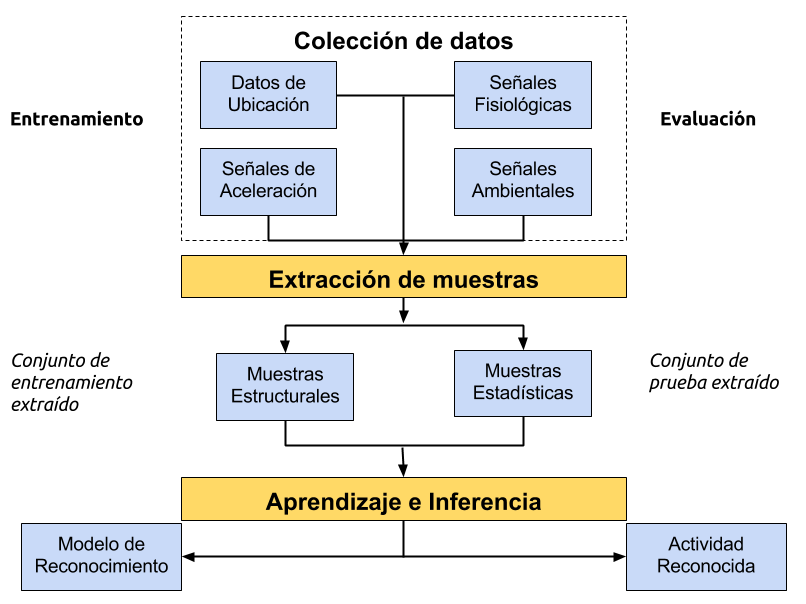
\includegraphics[width=0.7\linewidth]{capitulo-2/graphics/harsystem}
\caption[Flujograma\abbr{HAR}]{\label{fig2:harsystem}Flujo general del Reconocimiento de Actividades
Humanas}
 
\end{figure}

En la \figref{fig2:harsystem} se visualiza las fases comunes de estas
dos etapas\cite{LaraLabrador2013}. La etapa de entrenamiento requiere
inicialmente un conjunto de datos recolectados en una serie de tiempo
con los atributos medidos a partir de individuos que realizan cada
actividad. Las series se dividen en ventanas de tiempo para aplicar
la extracción de muestras filtrando así la información relevante de
las señales en bruto. 

Más adelante, se utilizan métodos de aprendizaje para generar un modelo
de reconocimiento de actividades a partir del conjunto de datos colectado
a través de las características calculadas. Del mismo modo, para la
etapa de prueba o evaluación, se recogen datos durante una ventana
de tiempo, que se utiliza para extraer las mismas características
utilizadas en el modelo, estas se evalúan en el modelo de aprendizaje
previamente entrenado, generando una etiqueta de la actividad predicha.

En las siguientes secciones detallamos las actividades humanas que
son objeto de la clasificación y las funciones de cada etapa.

\subsection{Actividades Humanas}

\label{sec263:actividades-humanas} El diseño e implementación de
un sistema \abbr{HAR} depende totalmente de las actividades que serán
reconocidas. Por lo tanto, el cambio del conjunto de actividades que
un sistema reconoce convierte al problema en uno completamente distinto
a otro sistema construido con el mismo propósito.

Teniendo en cuenta esta razón, y de acuerdo a distintas publicaciones,
presentamos siete grupos distintos de actividades agrupados en la
siguiente tabla.

\begin{table}[htbp]
\centering{}%
\begin{tabular}{|l|p{9cm}|}
\hline 
\textbf{Grupo}  & \textbf{Actividades} \tabularnewline
\hline 
\hline 
Ambulatoria  & Caminar, correr, sentarse, pararse, quedarse quieto, acostarse, subir
escaleras, descender escaleras, usar escaleras mecánicas, usar elevador.\tabularnewline
\hline 
Transporte  & Andar en bus, bicicleta y conducir \tabularnewline
\hline 
En el teléfono  & Enviar mensajes de texto y hacer llamadas \tabularnewline
\hline 
Actividades diarias  & Comer, beber, trabajar en la PC, observar TV, leer un libro, cepillarse
los dientes, aspirar el piso, y otros. \tabularnewline
\hline 
Ejercitarse  & Alzar pesas, bicicleta estática, remo y otros. \tabularnewline
\hline 
Militares  & Arrastrarse, en cuclillas, abrir la puerta \tabularnewline
\hline 
Parte superior del cuerpo  & Masticar, hablar, mover la cabeza, tragar líquidos, mirar. \tabularnewline
\hline 
\end{tabular}\caption[Grupos de Actividades]{\label{tab2:grupo-actividades}Grupos de Actividades}
\end{table}

Las actividades pueden separase en varios grupos de acuerdo a la duración
y la complejidad del evento. Los eventos cortos son movimientos de
transición y movimientos en base a gestos. Los eventos al que nos
enfocamos en este trabajo son aquellos que se componen de las actividades
básicas de larga duración que se caracterizan por las acciones continuas
y cíclicas de un individuo \cite{ReyesOrtiz2015}. Nuestro estudio
no se basa en actividades complejas que sean una secuencia de actividades
básicas y eventos cortos.

Definimos como objetivo de estudio detectar actividades básicas ambulatorias
y de transporte, de larga duración y sin cambios bruscos de transición.

\subsection{Colección de Datos}

La definición del método de colección de datos es un punto importante
en un sistema \abbr{HAR}. Según como se realiza la observación del
individuo, puede darse el caso de captura en ambientes realistas los
cuales son los ideales pero no siempre posibles, y también los ambientes
casi-realistas llevadas acabo en laboratorios donde se simula así
las condiciones reales de las actividades humanas. Por otro lado tenemos
los ambientes totalmente controlados en laboratorio.

Una falla en el diseño de un sistema \abbr{HAR} se puede dar por
no considerar las condiciones reales de las actividades, tales como
actividades no tenidas en cuenta, calibración de sensores, ruido,
etc. Otra de las consideraciones a tener en cuenta en este punto es
la cantidad de individuos para realizar la colección, es recomendable
el mayor cantidad de individuos en distintos tipos de edades y condiciones
físicas.

\subsection{Extracción de Muestras}

Para cualquier problema de aprendizaje automático, la selección de
características se refiere al proceso de selección de un conjunto
significativo de características que aporten relevancia a la capacidad
de discriminación en un algoritmo de aprendizaje. Por otro lado, la
extracción de características, tiene como objetivo disminuir la cantidad
de características a utilizar mediante distintas transformaciones
entre ellas para obtener nuevas características reducidas sin perder
información relevante del conjunto de datos originales. La selección
y extracción de características también permite reducir los tiempos
de procesamiento en la fase de entrenamiento y aumenta el rendimiento
en la fase de evaluación

Dependiendo de la aplicación, las características requeridas para
la extracción de la información relevante pueden variar. En el caso
particular de \abbr{HAR}, una representación reducida de los datos
del sensor se puede utilizar como la entrada del algoritmo de reconocimiento.
Esto se logra mediante medición de la señal del sensor en varios dominios,
pudiendo ser en tiempo y frecuencia.

\subsection{Aprendizaje e Inferencia}

Varios enfoques de aprendizaje automático se han desarrollado a lo
largo de los años para resolver el problema de \abbr{HAR}. En su
mayoría a través de algoritmos de aprendizaje supervisado aunque también
se han propuesto métodos semisupervisados y no supervisados.

La diferencia entre el aprendizaje supervisado y no supervisado consiste
en la utilización de datos etiquetados y no etiquetados respectivamente.
Debido a que el objetivo de un sistema \abbr{HAR} es encontrar una
actividad etiquetada como caminando, corriendo, quieto, etc., la mayoría
de los sistemas \abbr{HAR} utilizan un enfoque supervisado.

El aprendizaje automático supervisado, referido como clasificación
para problemas de clases discretas, ha sido un área bastante productiva
con varios algoritmos efectivos resumidos en la tabla \tabref{tab2:metodos-aprendizaje}.
Estas técnicas resuelven otras tareas además de la clasificación como
la regresión y el agrupamiento.

\begin{table}
\begin{centering}
\begin{tabular}{|>{\raggedright}m{4cm}|>{\raggedright}p{9cm}|}
\hline 
\textbf{Grupo}  & \textbf{Actividades} \tabularnewline
\hline 
\hline 
Basados en Reglas & Árboles de decisión (\abbr{DT}, \emph{Decision Trees})

Selvas aleatorias (\abbr{RF}, \emph{Random Forest})\tabularnewline
\hline 
Enfoques Geométricos  & Vecinos cercanos (\abbr{k-NN}, \emph{k Nearest Neighbourhood})

Redes neuronales (\abbr{ANN}, \emph{Artificial Neural Network})

Máquinas de soporte-vector (\abbr{SVM}, \emph{Support Vector Machines})\tabularnewline
\hline 
Clasificación Probabilista & Clasificadores de Bayes (\abbr{NB}, \emph{Naive Bayes}), 

Modelos de Markov (\abbr{HMM}, \emph{Hidden Markov Models})\tabularnewline
\hline 
\end{tabular}
\par\end{centering}
\caption[Métodos de aprendizaje agrupados]{\label{tab2:metodos-aprendizaje}Resumen de métodos de aprendizaje
agrupados por tipo}
\end{table}

Los aspectos relevantes para la selección de un algoritmo de aprendizaje
pueden ser: el consumo de energía, los requisitos de memoria, la complejidad
de computo e interpretación, etc. Estos aspectos se agudizan si se
utilizan dispositivos móviles inteligentes. Por ejemplo, los árboles
de decisión podría ser el método preferido cuando se requiere simplicidad
en la implementación y métodos \abbr{SVM} para aplicaciones que requieran
un alto rendimiento pero con mayor complejidad\cite{ReyesOrtiz2015}.

En el capitulo \ref{chap3:Aprendizaje-Automatico} se detalla la base
teórica referente a las técnicas de aprendizaje automático supervisados
y el método de árboles de decisión electo para este trabajo.

\section{Conclusión}

\label{sec27:conclusion}Este capitulo abarcó los tópicos primordiales
del estudio del reconocimiento de las actividades humanas. Los conceptos
descritos sirven de base de conocimiento para entender el problema
de \abbr{HAR} y además permiten tener una vista general de los componentes
principales para resolver el problema. Primeramente se cubre la motivación
en base a las aplicaciones, luego los medios disponibles para construir
estos sistemas: sensores, teléfonos móviles y aprendizaje automático,
y finalmente la definición metodológica y teórica del problema. 
